\section{Activation Functions}
\label{appendix:activations}

ReLU (Rectified Linear Unit), Leaky ReLU (with gradient parameter $\alpha$) and tanh activation functions are depicted in Figure \ref{fig:activation_functions}. They can also be expressed mathematically as:
\begin{align*}
    \text{ReLU}(x) &= \max(0, x) \\
    \text{Leaky ReLU}(x) &= \begin{cases} 
        x & \text{if } x \geq 0 \\ 
        \alpha x & \text{if } x < 0 
    \end{cases} \\
    \text{tanh}(x) &= \frac{e^x - e^{-x}}{e^x + e^{-x}}
\end{align*}

\begin{figure}[h]
  \centering
  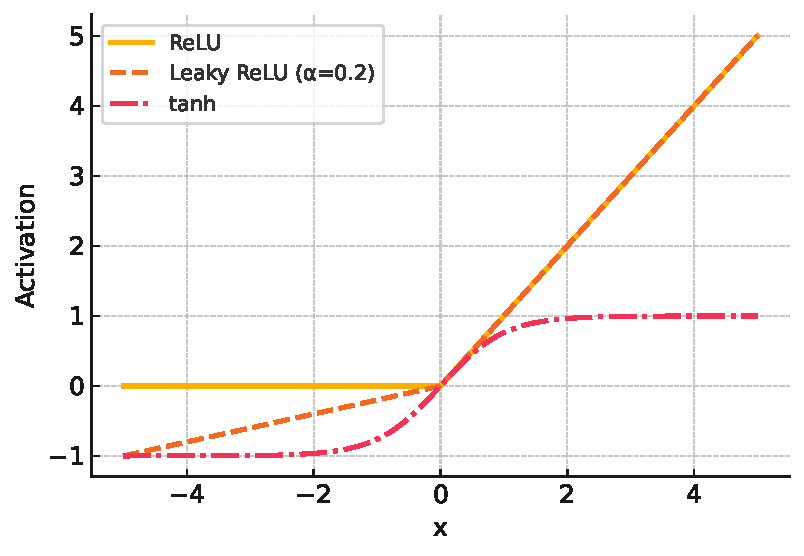
\includegraphics[width=0.6\textwidth]{Images/activations_visible.pdf}
  \caption{Comparison of ReLU, Leaky ReLU, and tanh activation functions.}
  \label{fig:activation_functions}
\end{figure}